\documentclass{article}
\usepackage[a4paper, margin=3cm]{geometry}
\usepackage{graphicx}
\usepackage{algorithm}
\usepackage{algpseudocode}
\usepackage{hyperref}
\usepackage{comment}
\usepackage{amsmath}
\usepackage{enumitem}
\usepackage{amsfonts}
\usepackage{tikz}
\usetikzlibrary{arrows.meta,positioning,fit,calc}
\usepackage{rotating}

\newtheorem{theorem}{Theorem}[section]   % numbered per section
\newtheorem{lemma}[theorem]{Lemma}       % shares numbering with theorem
\newtheorem{corollary}[theorem]{Corollary}
\newtheorem{definition}[theorem]{Definition}
\usepackage{titling}

% Title formatting
\pretitle{\centering\LARGE\bfseries\vspace{0em}}
\posttitle{\par\vspace{1em}}

\preauthor{\centering\large}
\postauthor{\par\vspace{1em}}

\predate{\centering\small}
\postdate{\par}


\setlength{\parindent}{0pt} % no indend automatically everywhere

\title{Project Report\\Binary Heap and Dijkstra's Algorithm}
\author{
	\centering
	Josefine Lindmar
	Sonja Joost
}
\date{\today} % empty date



\begin{document}

\maketitle

\section{Introduction}
TODO Brief overview and motivation

\section{Binary Heap}
\textbf{Goal.} The goal of the binary heap part of the project is to formalize the binary heap together with the operations needed for the Dijstra algorithm. This included the following:
\begin{itemize}
    \item \texttt{heapify}: Create a heap from a given array
    \item \texttt{insert}: Add a new key to the heap and restore the binary heap invariant by bubbling the element to its correct position.
    \item \texttt{extract-min (/max)}: Pop the minimum (resp. maximum) element from the heap and restore the binary heap invariant by placing a leaf node at the root and trickling it down to the position it belongs.
    \item \texttt{decrease-key (/increase-key)}: Decrease (resp. increase) the value of an element’s key to the new value, which is assumed to be less than or equal to the current key's value and restoring the heap invariant such that the node is at the correct position according to its new value.
\end{itemize}

\subsection*{Data Structure}

A binary heap is a data structure that represents data as a nearly complete binary tree \cite{clrs}. The binary heap must satisfy the heap condition, which depends on the type of heap. There are min and max heaps, where the root is the smallest or highest value, respectively. In a min heap, the value of each node is less than or equal to its parent's value. In a max heap, the value of each node is greater than or equal to its parent's value.


A binary heap as two possible representations. It can be viewed as a binary tree as well as an array that is structured as binary tree through the indices. As the binary tree representation allows for a straight forward possibility to perform structural induction, we chose to take a binary heap as underlying data structure for the binary heap.
\newline

\small
\texttt{inductive BinaryTree (}\(\alpha\)\texttt{ : Type)}\\
\texttt{| leaf : BinaryTree }\(\alpha\)\\
\texttt{| node : BinaryTree }\(\alpha\)\texttt{ $\to$ }\(\alpha\)\texttt{ $\to$ BinaryTree }\(\alpha\)\texttt{ $\to$ BinaryTree }\(\alpha\)
\vspace{3mm}
\newpage

We chose to allow a the binary heap to be of any type $\alpha$. As we will later see, there are some restrictions on $\alpha$ needed for the implementation of some operations. The values of the nodes are assigned by a function $f$ that is passed along with the binary tree. $f$ assigns to each node a value of type \texttt{ENat}. \texttt{ENat} allows for the representation of infinity which is needed for the Dijksta algorithm.
The binary min heap invariant is then defined as a proposition on the binary tree that holds whenever all nodes have a smaller value assigned to by $f$ than its parents:
 \newline
 
\texttt{def is\_min\_heap : BinaryTree }$\alpha$\texttt{ → (ordering : }$\alpha$\texttt{ → ENat) → Prop}\\
\texttt{| leaf, \_ => true}\\
\texttt{| node l v r, f => match l, r with}\\
\quad\texttt{| leaf, leaf => true}\\
\quad\texttt{| node \_ lv \_, leaf => f v }$\le $\texttt{ f lv }$\wedge$\texttt{ isMinHeap l f}\\
\quad\texttt{| leaf, node \_ rv \_ => f v }$ \le $\texttt{ f rv }$\wedge$\texttt{ isMinHeap r f}\\
\quad\texttt{| node \_ lv \_, node \_ rv \_ =>}\\
\qquad\texttt{ f v } $\le $\texttt{ f lv }$\wedge$\texttt{ isMinHeap l f }$\wedge$\texttt{}
\texttt{ f v }$ \le$ \texttt{ f rv }$\wedge$\texttt{ isMinHeap r f}\\
\vspace{3mm}


\subsection{Operations}
For the operations on the binary heap, we show that they function as expected. In particular, we show that the functionality is correct and the binary heap invariant is established (or preserved, respectively).
\subsubsection{heapify}
Heapify is a subroutine that is used by several of the operations. It takes a binary tree as input for which the heap invariant holds for both of its children if they exist and moves the root node to the correct position such that the heap invariant holds for the whole binary tree. We show for the formalization that it establishes the heap invariant and the output contains the exact same nodes as the input. We formulate the theorem to be over general trees (as opposed to only nodes that have children) to be able to perform induction in the proof. In particular:
\\

\textbf{Theorem. Correctness \texttt{heapify}.}
Let $bt$ be a binary tree over elements of type $\alpha$, and let $f: \alpha \to \mathbb{N} \cup \{\infty\}$ be a function. Then:
 \begin{align}  
&(\forall v. v \in bt \iff v \in \texttt{heapify}(bt, f)) \land \\
&(\exists l, v, r. bt = \texttt{node} (l, v, r) \Rightarrow \texttt{is\_min\_heap}(l, f) \land \texttt{is\_min\_heap}(r, f) \Rightarrow  \texttt{is\_min\_heap}(\texttt{heapify}(bt, f), f))
 \end{align}
\\
\textbf{English explanation.} To prove the first part, we just show that no node was added or removed during the heapify operation. The second part requires a proof by functional induction over \texttt{heapify}. The base cases are trivial as the \texttt{leaf} and the node with only \texttt{leafs} as children satisfy the heap invariant by definition. The cases that don't call \texttt{heapify} recursively can be solved with the definition and the assumptions availiable at the respective proof states. For the other three cases, the structure of the proof is similar: We use the fact that a binary tree satisfies the heap condition if both children are min heaps and the value assigned the root node is less of equal to the one of the children. This allows us to use the induction hypothesis for the two children and we are able to use the conditions for the cases to show that the root indeed holds the minimum value.


\textbf{Lean correspondence.}
We show both statements separately. We split the first one into the both directions (\texttt{contains\_then\_heapify\_contains, heapify\_contains\_then\_contains}) and can prove both with functional induction over \texttt{heapify} and the definition of \texttt{contains} (which corresponds to $\in$).
We do \texttt{fun\_induction heapify generalizing l r v; all\_goals expose\_names}. Note that we need to generalize the induction hypothesis in order to apply it to the children of the tree. For the leaf cases and the ones that do not recurs, we can simply use the definition of heapify together with the assumptions. For the cases that call \texttt{heapify}, we define a helper lemma that shows that if the two children are min heaps and the value assigned to the root is less than or equal to that of the children, then the tree is a min heap (\texttt{left\_and\_right\_are\_min\_heap\_and\_root\_is\_min\_of\_children\_is\_min\_Heap}). To show that the children are min heaps we can simply use the induction hypothesis (as the children are min heaps, its children are also min heaps, so the induction hypothesis can be applied (by \texttt{min\_heap\_then\_left\_and\_right\_are\_min\_heap})) and the assumptions. To show that the root value is smaller that the values of the children, we use the fact, that in the \texttt{heapify} we switch the root with the smaller child if it is larger and then, the smallest value of each of the children is smaller than the root because the children are min heaps (\texttt{root\_is\_min\_of\_children, min\_heap\_member\_le\_root}) and its members did not change except for the potentially switched root whose value is larger (\texttt{heapify\_contains\_then\_contains}).

\subsubsection{insert}
...
\\

\textbf{Theorem. Correctness \texttt{insert}.}
Let $bt$ be a binary tree over elements of type $\alpha$, and let $f: \alpha \to \mathbb{N} \cup \{\infty\}$ be a function. Then:
 \begin{align}  
...
 \end{align}
\\
\textbf{English explanation.}
\\
\textbf{Lean correspondence.}

\subsubsection{extract-min}
\textbf{Theorem. Correctness \texttt{extract-min}.}
Let $bt$ be a binary tree over elements of type $\alpha$, and let $f: \alpha \to \mathbb{N} \cup \{\infty\}$ be a function. Then:
 \begin{align}  
...
 \end{align}
\\
\textbf{English explanation.}
\\
\textbf{Lean correspondence.}

\subsubsection{decrease-key}
\textbf{Theorem. Correctness \texttt{decrease-key}.}
Let $bt$ be a binary tree over elements of type $\alpha$, and let $f: \alpha \to \mathbb{N} \cup \{\infty\}$ be a function. Then:
 \begin{align}  
...
 \end{align}
\\
\textbf{English explanation.}
\\
\textbf{Lean correspondence.}


\section{Dijkstra's algorithm}
\textbf{Goal.} Formalize Dijkstra's algorithm over finite graphs and prove correctness, using a priority queue abstraction. Our Lean development lives in \texttt{Projects/Lindmar\_Joost/Dijkstra.lean}.\\

We represent the graph as a finite simple graph so vertices have decidable equality (exactly how we have seen it in the BinarySort examples in class). Distances use extended natural numbers (so an unknown distance can be “infinity”), called \texttt{ENat} in Lean. The algorithm state is just a pair: a distance map from vertices to these extended naturals (\(\texttt{dist} : V \to \mathbb{N}_\infty\)) and a binary-heap priority queue (\(\texttt{queue} : \texttt{BinaryHeap}\)). The heap exposes abstract operations (empty check, extract-min, decrease-priority, size) and the proofs only rely on their contracts. 

The algorithm is split up into three parts: 
\begin{itemize}
	\item Relaxation (Lean: \texttt{relaxNeighbors}) is a simple loop over the neighbors of a vertex u that updates each neighbor v by setting $dist(v)$ to the minimum of its current value and $dist(u)+1$, and it conceptually decreases v’s priority in the heap when that happens.
	\item The recursive core of Dijkstra (Lean: \texttt{dijkstra\_rec}) repeatedly extracts the current minimum u, relaxes u’s neighbors (updating the distance map and heap), and then recurses on the new state.
	\item The top-level function (Lean: \texttt{dijkstra}) initializes distances with 0 at the source and infinity elsewhere, inserts the source into the heap, and starts the recursion.
\end{itemize}



\subsection*{Termination}
We split the implementation into three parts: \texttt{dijkstra} (a non-recursive wrapper), \texttt{dijkstra\_rec} (the recursive core), and \texttt{relaxNeighbors} (implemented as a fold over the finite list of neighbors). Hence termination needs to be shown only for \texttt{dijkstra\_rec}: \texttt{dijkstra} is trivially terminating because it does not recurse, and \texttt{relaxNeighbors} terminates by structural recursion on a finite list (Lean accepts it as a terminating fold), so no additional termination proof is required for them.

We prove termination by the measure \texttt{queue.sizeOf}: if \texttt{queue.isEmpty} the recursion stops, otherwise extracting the minimum yields \texttt{(u, queue')} and \texttt{BinaryHeap.sizeOf\_extract\_min\_lt\_of\_isEmpty\_eq\_false} gives \(\texttt{queue'.sizeOf} < \texttt{queue.sizeOf}\); since \texttt{relaxNeighbors} does not increase the heap size the post-relax queue has strictly smaller size than the original, so the \texttt{queue.sizeOf} measure decreases on every recursive call. In Lean this is written as \texttt{termination\_by queue.sizeOf} and discharged by applying \texttt{BinaryHeap.sizeOf\_extract\_min\_lt\_of\_isEmpty\_eq\_false} plus the trivial bookkeeping to turn the hypothesis into the expected \texttt{isEmpty = false} form.


\subsection*{Correctness proof (\texorpdfstring{$\texttt{dijkstra\_correctness}$}{dijkstra\_correctness})}
\emph{Statement.} For any vertex \(v\), the algorithm’s output equals the graph distance $\delta$: \[(\texttt{dijkstra}\ g\ s\ v)\ v = \delta(g,s,v)\]

The proof proceeds by fixing the algorithm's output and deriving a contradiction from any alleged disagreement with the true graph distance. Concretely, set
\[
\texttt{dist} := \texttt{dijkstra}\ g\ s\ v
\]
(in Lean: \texttt{set dist := (dijkstra g s v) with hdist}). First establish the global lower bound
\[
\forall u,\ \delta(s,u)\le \texttt{dist}\ u,
\]
provided by the lemma \texttt{neverUnderestimates}. Note also that \(\delta(s,s)=0\) and by \texttt{dijkstra\_source\_zero} the algorithm assigns \(0\) to the source, so any counterexample cannot be the source.

Assume, for contradiction, that there exists a vertex \(u\) with \(\texttt{dist}\ u \ne \delta(s,u)\). Choose such a \(u\) that minimizes \(\delta(s,u)\) (Lean: \texttt{minimalCounterexample}). By the previous remark we have \(\delta(s,u)>0\), so take a shortest path from \(s\) to \(u\); this yields a predecessor \(y\) with \(y\sim u\) and
\[
\delta(s,u)=\delta(s,y)+1
\]
(Lean: \texttt{existsPredOnShortestPath}). By minimality of \(u\) we have \(\delta(s,y)<\delta(s,u)\), hence \(\texttt{dist}\ y=\delta(s,y)\).

Now apply the algorithmic per-edge final bound \texttt{relaxAdj\_final\_bound} to the edge \(y\sim u\). That lemma (which internally uses \texttt{exists\_extract\_or\_top}, \texttt{relaxNeighbors\_adj\_upper}, and the \(y\)-stability lemmas such as \texttt{extracted\_value\_is\_final\_lemma}) yields
\[
\texttt{dist}\ u \le \texttt{dist}\ y + 1.
\]
Substituting \(\texttt{dist}\ y=\delta(s,y)\) and \(\delta(s,y)+1=\delta(s,u)\) gives \(\texttt{dist}\ u \le \delta(s,u)\). Together with the global lower bound \(\delta(s,u)\le \texttt{dist}\ u\) this forces equality \(\texttt{dist}\ u = \delta(s,u)\), contradicting the choice of \(u\).

Hence no counterexample exists, and we conclude \texttt{dijkstra\_correctness}: for every vertex \(v\) the algorithm's output equals the graph distance \(\delta(g,s,v)\).
\paragraph{Preconditions and placeholders.}
The development assumes the standard BinaryHeap contracts and builds the correctness proof from a number of named lemmas, many of which in turn rely on smaller auxiliary facts. Figure~\ref{fig:dijkstra-deps} illustrates the dependency relation between the main lemmas used in this file; For space and clarity some minor lemmas are not shown in the diagram. 

All of the lemmas have been fully formalized except for the search lemma \texttt{exists\_extract\_or\_top}, which is currently left as a \texttt{sorry}, and the lower bound leamm \texttt{neverUnderestimates}. A discussion of why those particular proof remain unfinished appears in the "Main Challenges" section at the end of the report.

\begin{sidewaysfigure}
\centering
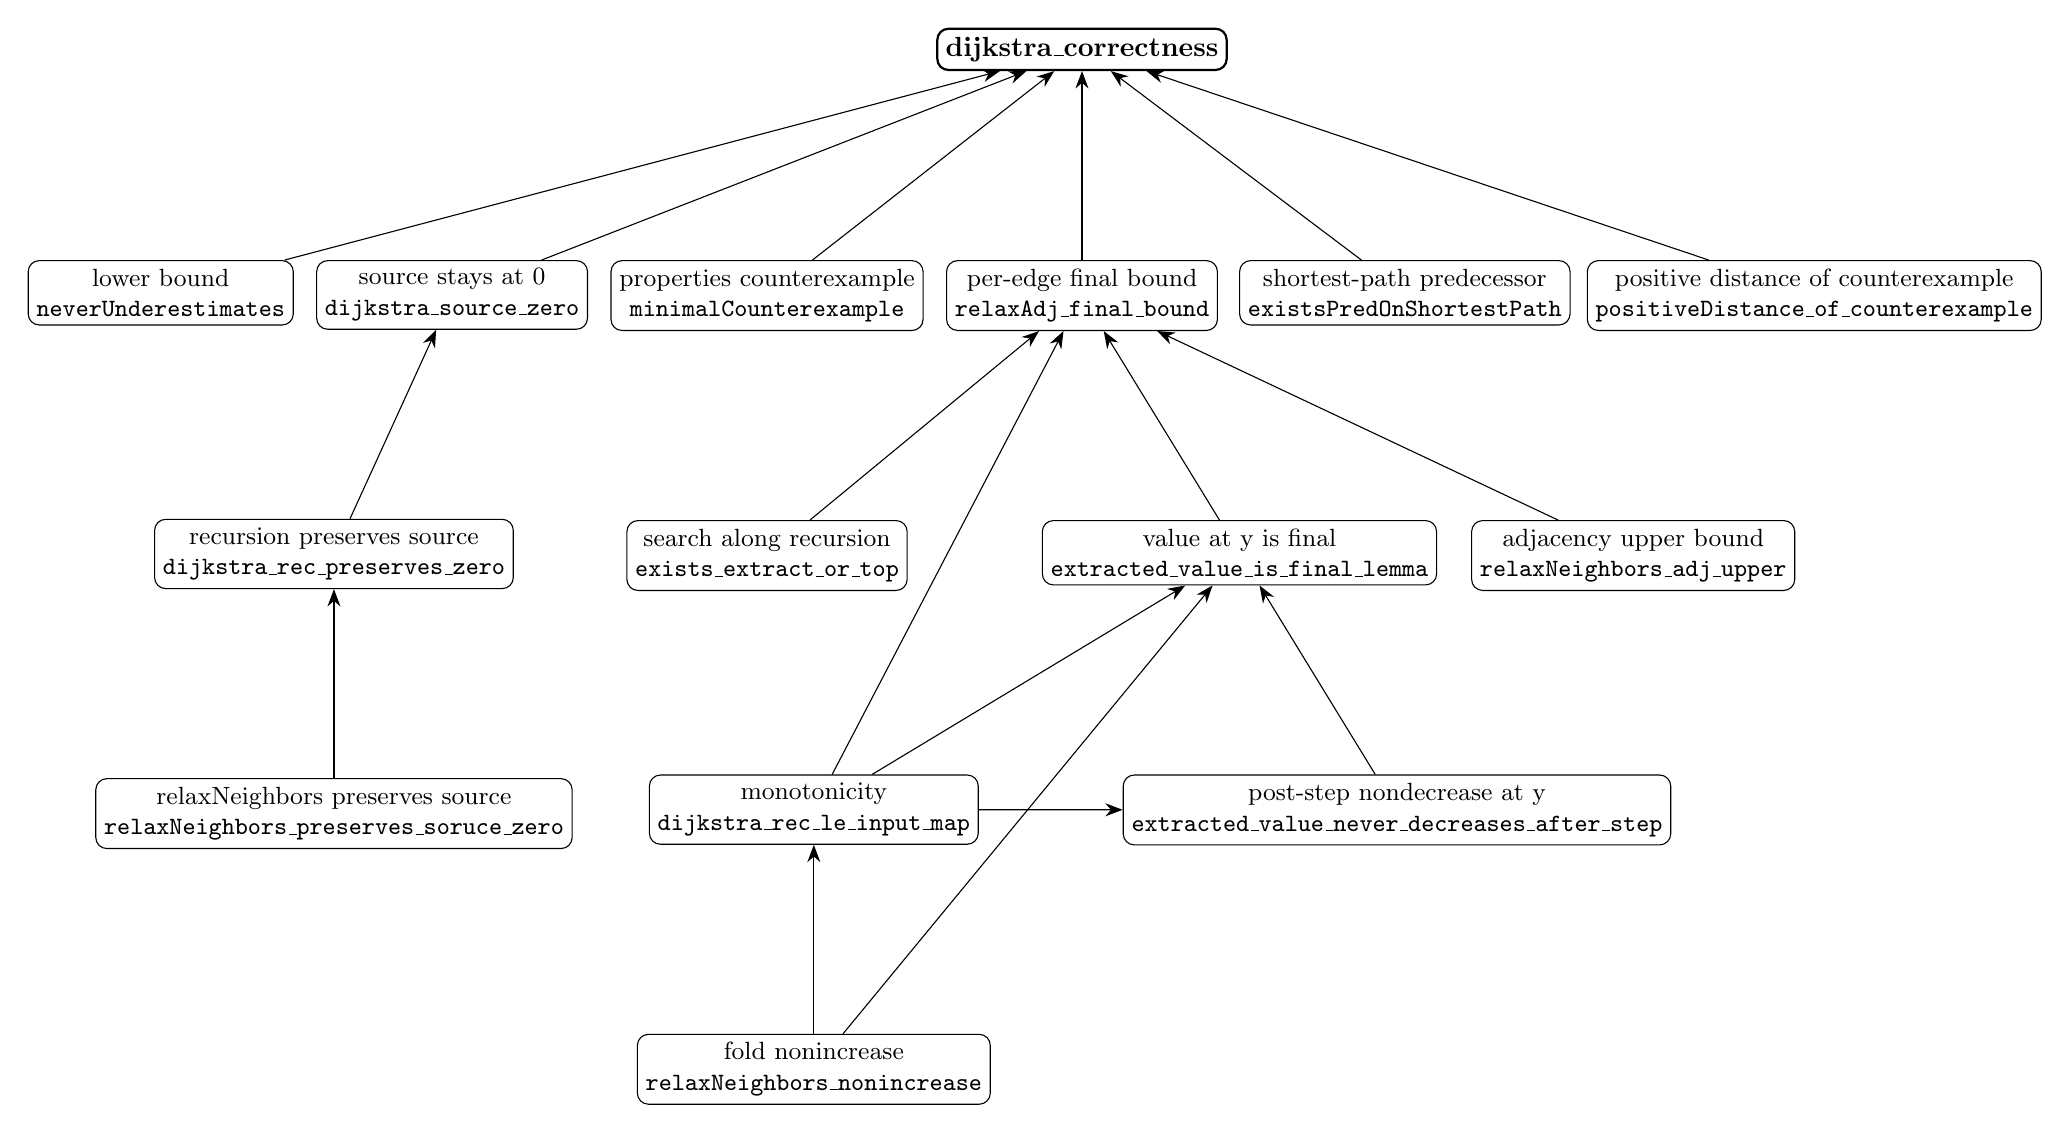
\begin{tikzpicture}[
  node distance=10mm and 12mm,
  box/.style={rectangle, draw, rounded corners, align=center, inner sep=3pt, font=\small},
  grp/.style={draw, rounded corners, inner sep=4pt, dashed},
  >={Stealth[length=2.2mm]},
  every edge/.style={draw, -{Stealth[length=2.2mm]}}
]
% Top layer: correctness
\node[box, font=\normalsize, thick] (CORR) {\textbf{dijkstra\_correctness}};

\node[box, below=24mm of CORR, xshift=-117mm] (LOWER) {lower bound\\\texttt{neverUnderestimates}};
\node[box, below=24mm of CORR, xshift=-80mm] (ZERO_TOP) {source stays at 0\\\texttt{dijkstra\_source\_zero}};
\node[box, below=24mm of CORR, xshift=-40mm] (CNT) {properties counterexample\\\texttt{minimalCounterexample}};
\node[box, below=24mm of CORR, xshift=0mm] (EDGE) {per-edge final bound\\\texttt{relaxAdj\_final\_bound}};
\node[box, below=24mm of CORR, xshift=41mm] (PRED) {shortest-path predecessor\\\texttt{existsPredOnShortestPath}};
\node[box, below=24mm of CORR, xshift=93mm] (CNT_DIST) {positive distance of counterexample\\\texttt{positiveDistance\_of\_counterexample}};

% Edges: correctness
\path (LOWER) edge (CORR);
\path (CNT) edge (CORR);
\path (ZERO_TOP) edge (CORR);
\path (CNT_DIST) edge (CORR);
\path (PRED) edge (CORR);
\path (EDGE) edge (CORR);

% LEVEL 2 (wider spacing to avoid horizontal overlap)
\node[box, below=24mm of EDGE, xshift=-40mm] (SEARCH) {search along recursion\\\texttt{exists\_extract\_or\_top}};
\node[box, below=24mm of EDGE, xshift=20mm]   (EVF)    {value at y is final\\\texttt{extracted\_value\_is\_final\_lemma}};
\node[box, below=24mm of EDGE, xshift=70mm]  (RAU)    {adjacency upper bound\\\texttt{relaxNeighbors\_adj\_upper}};
% Edges toward EDGE (per-edge final bound)
\path (SEARCH) edge (EDGE);
\path (EVF) edge (EDGE);
\path (RAU) edge (EDGE);

\node[box, below = 24mm of ZERO_TOP, xshift=-15mm] (ZERO_MIDDLE) {recursion preserves source\\\texttt{dijkstra\_rec\_preserves\_zero}};
\path (ZERO_MIDDLE) edge (ZERO_TOP);


% LEVEL 3
\node[box, below left=24mm and 8mm of EVF] (MONO) {monotonicity\\\texttt{dijkstra\_rec\_le\_input\_map}};
\node[box, below=24mm of EVF, xshift=20mm] (EVND) {post-step nondecrease at y\\\texttt{extracted\_value\_never\_decreases\_after\_step}};
\path (MONO) edge (EVF);
\path (MONO) edge (EDGE);
\path (MONO) edge (EVND);
\path (EVND) edge (EVF);

\node[box, below = 24mm of ZERO_MIDDLE] (ZERO_BOTTOM) {relaxNeighbors preserves source\\\texttt{relaxNeighbors\_preserves\_soruce\_zero}};
\path (ZERO_BOTTOM) edge (ZERO_MIDDLE);

% LEVEL 4
\node[box, below=24mm of MONO] (RNI) {fold nonincrease\\\texttt{relaxNeighbors\_nonincrease}};
\path (RNI) edge (MONO);
\path (RNI) edge (EVF);







% Group annotations (optional dashed boxes)
%\node[grp, fit=(RNI) (RAU), label={[align=center]below:{\footnotesize Relaxation facts}}] {};
%\node[grp, fit= (EVND) (EVF), label={[align=center]right:{\footnotesize Stability at $y$}}] {};

\end{tikzpicture}
\caption{Lemma dependency graph shaping the proof of correctness.}
\label{fig:dijkstra-deps}
\end{sidewaysfigure}

\newpage


\subsection*{Lower bound (\texttt{neverUnderestimates})}
\textbf{Statement.} For any vertex \(u\), Dijkstra's output never underestimates the true graph distance: \[(\texttt{dijkstra}\ g\ s\ t)\ u \ge \delta(g,s,u)\]

This lemma establishes a global lower bound on the algorithm's output. In the Lean file, \texttt{neverUnderestimates} is currently left as \texttt{admit}. All online references we found assume this property as a given, and formalizing it requires reasoning about graph walks and path induction with Mathlib's \texttt{SimpleGraph.Walk} machinery, which was beyond the scope of this project. We therefore treat this lemma as an axiomatic starting point for our correctness proof.

\subsection*{Source preservation (\texttt{dijkstra\_source\_zero}, \texttt{dijkstra\_rec\_preserves\_zero}, \texttt{relaxNeighbors\_preserves\_source\_zero})}
\textbf{Statement.} The source vertex \(s\) always maintains distance \(0\) throughout the algorithm: \[(\texttt{dijkstra}\ g\ s\ t)\ s = 0\]

\textbf{English explanation.} Dijkstra initializes \(\texttt{dist}(s) = 0\) and \(\texttt{dist}(v) = \top\) for all \(v \ne s\). We must show that this invariant is preserved through all recursive steps. The key observation is that \texttt{relaxNeighbors} only updates neighbors of the extracted vertex \(u\), and each update sets a neighbor's distance to \(\texttt{dist}(u)+1\). Since the graph is simple (irreflexive), \(s\) is never a neighbor of itself, so it can only be updated if it appears as a neighbor of some other vertex \(u\). But even if \(s\) were a neighbor of \(u\), the update condition \(\texttt{dist}(u)+1 < \texttt{dist}(s)\) would require \(\texttt{dist}(u)+1 < 0\), which is impossible in extended naturals. Therefore \(\texttt{dist}(s)\) remains unchanged at \(0\) after every relaxation step, and by induction on the recursion depth (using strong induction on the heap size), it stays \(0\) in the final output.

\textbf{Lean correspondence.} The proof is split into three lemmas in a bottom-up fashion. \\
\texttt{relaxNeighbors\_preserves\_source\_zero} proves preservation for a single relaxation step by unfolding the fold over neighbors and showing that the update branch never triggers for the source (the condition \(\texttt{dist}(u)+1 < 0\) is false, which we encode as \texttt{enat\_add\_one\_not\_lt\_zero}). We proceed by induction on the neighbor list, proving that each step preserves \(\texttt{dist}(s)=0\). Next, \texttt{dijkstra\_rec\_preserves\_zero} lifts this to the full recursion via strong induction on \texttt{sizeOf(queue)}: if the queue is empty the result is immediate; otherwise we extract \(u\), apply the previous lemma to get \(\texttt{dist}'(s)=0\) after relaxation, then apply the induction hypothesis to the smaller post-step heap. Finally, \texttt{dijkstra\_source\_zero} invokes the recursive lemma on the initial state.

\subsection*{Minimal counterexample (\texttt{minimalCounterexample}, \\\texttt{positiveDistance\_of\_counterexample})}
\textbf{Statement.} If there exists a vertex where Dijkstra's output disagrees with the true distance, then among all such counterexamples there exists one \(u\) with minimal \(\delta(s,u)\), and moreover for every \(w\) with \(\delta(s,w) < \delta(s,u)\), we have \(\texttt{dist}(w) = \delta(s,w)\). Furthermore, any such minimal counterexample must satisfy \(\delta(s,u) > 0\), i.e., \(u \ne s\).

\textbf{English explanation.} This is a standard proof-by-contradiction setup. We assume for contradiction that the set \(S\) of counterexamples (vertices where \(\texttt{dist}(u) \ne \delta(s,u)\)) is nonempty. Since the vertex set is finite, we can pick an element \(u \in S\) that minimizes \(\delta(s,u)\) over all counterexamples. By definition of minimality, any vertex \(w\) with strictly smaller distance must not be a counterexample, hence \(\texttt{dist}(w) = \delta(s,w)\). The second part shows that \(u \ne s\) because the source is correctly initialized to distance \(0\), which matches \(\delta(s,s)=0\), so the source cannot be a counterexample. Therefore \(\delta(s,u) > 0\).

\textbf{Lean correspondence.} \texttt{minimalCounterexample} formalizes the minimality argument. We define \(S\) as \texttt{Finset.univ.filter} on the predicate \(\texttt{dist}\ u \ne \delta\ g\ s\ u\), prove \(S\) is nonempty using the hypothesis, and apply \texttt{Finset.exists\_min\_image} to obtain a vertex \(u \in S\) minimizing \(\delta(s,\cdot)\). The minimality property follows by showing that if any \(w\) satisfies \(\delta(s,w) < \delta(s,u)\) and were also a counterexample, then \(\delta(s,u) \le \delta(s,w)\) by the minimality of \(u\), contradicting the strict inequality. The auxiliary lemma \texttt{positiveDistance\_of\_counterexample} uses the hypothesis \(u \ne s\) and connectivity of the graph to invoke Mathlib's \texttt{SimpleGraph.Reachable.dist\_eq\_zero\_iff}, which states that \(\delta(s,u)=0\) if and only if \(u=s\). Since \(u \ne s\), we have \(\delta(s,u) \ne 0\), hence \(\delta(s,u) > 0\).

\subsection*{Shortest-path predecessor (\texttt{existsPredOnShortestPath})}
\textbf{Statement.} If \(\delta(s,u) > 0\), there exists a vertex \(y\) adjacent to \(u\) such that \(\delta(s,u) = \delta(s,y)+1\).

\textbf{English explanation.} This lemma captures the simple fact that if \(u\) is not the source, any shortest path from \(s\) to \(u\) must traverse at least one edge, and the last edge of such a path provides the desired predecessor. Concretely, take a shortest walk \(p\) from \(s\) to \(u\) with \(p.\texttt{length} = \delta(s,u)\). Reverse it to obtain a walk from \(u\) to \(s\). Since \(\delta(s,u)>0\), this reversed walk is nonempty and begins with an edge from \(u\) to some vertex \(y\). The tail of this reversed walk is a walk from \(y\) to \(s\) of length \(\delta(s,u)-1\), hence \(\delta(s,y) \le \delta(s,u)-1\). Conversely, the triangle inequality and the edge \(y \sim u\) give \(\delta(s,u) \le \delta(s,y)+1\). Combining these yields equality.

\textbf{Lean correspondence.} The proof uses Mathlib's \texttt{SimpleGraph.Walk} API. We first invoke \texttt{SimpleGraph.Reachable.exists\_walk\_length\_eq\_dist} to obtain a shortest walk \(p : \texttt{Walk}\ s\ u\). We then case-analyze \texttt{p.reverse}: if it's \texttt{nil}, the length is zero, contradicting \(\delta(s,u)>0\); otherwise it's a \texttt{cons} with head adjacency \(u \sim y\) and a tail walk from \(y\) to \(s\). We compute that the reversed walk's length equals \(\texttt{tail.length}+1 = \delta(s,u)\), so \(\texttt{tail.length} = \delta(s,u)-1\). Since distance is the infimum of walk lengths, \(\delta(s,y) \le \texttt{tail.length}\), giving \(\delta(s,y)+1 \le \delta(s,u)\). The reverse inequality \(\delta(s,u) \le \delta(s,y)+1\) comes from the triangle inequality (formalized as \texttt{delta\_adj\_step\_ENat}). Antisymmetry yields equality.

\subsection*{Monotonicity (\texttt{dijkstra\_rec\_le\_input\_map})}
\textbf{Statement.} For any vertex \(x\), the recursive Dijkstra function never increases distances: \[(\texttt{dijkstra\_rec}\ g\ s\ t\ \texttt{dist}\ \texttt{queue})\ x \le \texttt{dist}\ x\]

\textbf{English explanation.} This lemma formalizes the intuitive property that relaxation steps can only improve (decrease) distance estimates, never worsen them. We prove it by strong induction on \(\texttt{sizeOf(queue)}\). If the queue is empty, \texttt{dijkstra\_rec} returns \(\texttt{dist}\) unchanged, so the inequality is trivial. Otherwise, we unfold one recursion step: extract the minimum vertex \(u\), relax its neighbors to obtain a new distance map \(\texttt{dist}'\) and queue \(\texttt{queue}'\), then recurse. The heap size strictly decreases after extraction and does not increase during relaxation, so \(\texttt{sizeOf(queue)'} < \texttt{sizeOf(queue)}\). By the induction hypothesis applied to the smaller heap, the final result satisfies \((\texttt{dijkstra\_rec}\ \cdots\ \texttt{dist}'\ \texttt{queue}')\ x \le \texttt{dist}'\ x\). The pointwise nonincrease property of \texttt{relaxNeighbors} gives \(\texttt{dist}'\ x \le \texttt{dist}\ x\). Composing these two inequalities via transitivity yields the desired bound.

\textbf{Lean correspondence.} The proof structure mirrors the English argument. We generalize the heap size to a parameter \(n\), revert the state variables, and apply \texttt{Nat.strong\_induction\_on}. The base case handles \texttt{queue.isEmpty = true} trivially. In the inductive step, we bind the extraction result with \texttt{let} statements (\texttt{step}, \texttt{u}, \texttt{queue'}, \texttt{next}) and apply two size lemmas: \texttt{BinaryHeap.sizeOf\_extract\_min\_lt\_of\_isEmpty\_eq\_false} for the strict decrease and \texttt{sizeOf\_relaxNeighbors\_le} for the nonincrease. The induction hypothesis then applies to the strictly smaller post-step heap size. Finally, \texttt{relaxNeighbors\_nonincrease} provides the one-step inequality \(\texttt{dist}'\ x \le \texttt{dist}\ x\), and we compose with \texttt{le\_trans}.

\subsection*{Relaxation properties (\texttt{relaxNeighbors\_nonincrease}, \texttt{relaxNeighbors\_adj\_upper})}
\textbf{Statement (nonincrease).} For all vertices \(x\), \[(\texttt{relaxNeighbors}\ g\ u\ \texttt{dist}\ q).1\ x \le \texttt{dist}\ x\]

\textbf{English explanation.} Relaxation is a fold over the neighbor list of \(u\). At each step, for a neighbor \(v\), we compute \(\texttt{alt} = \texttt{dist}(u)+1\) and conditionally update \(\texttt{dist}(v)\) to \(\min(\texttt{dist}(v), \texttt{alt})\). If the update happens, \(\texttt{dist}(v)\) decreases; otherwise it stays the same. Vertices other than the current neighbor are untouched in that step. By induction on the neighbor list, every coordinate of the distance map either decreases or stays the same, hence the final map is pointwise \(\le\) the input map.

\textbf{Lean correspondence.} We prove \texttt{relaxNeighbors\_nonincrease} by induction on the neighbor list. The fold function \(f\) is unfolded explicitly: if \(\texttt{alt} < \texttt{dist}(v)\), we set \(\texttt{dist}'(x) = \texttt{alt}\) for \(x=v\) and \(\texttt{dist}(x)\) otherwise; else the map is unchanged. The base case (empty list) is trivial. In the inductive step, we show that one application of \(f\) preserves the nonincrease property: for any \(x\), \(f(\texttt{dist},q)\ v\) yields a map with \(\texttt{dist}'(x) \le \texttt{dist}(x)\). We then apply the induction hypothesis to the tail of the list and compose the inequalities.




\textbf{Statement (adjacency upper bound).} If \(y \sim u\), then \[(\texttt{relaxNeighbors}\ g\ y\ \texttt{dist}\ q).1\ u \le \texttt{dist}(y)+1\]

\textbf{English explanation.} When relaxing neighbors of \(y\), the vertex \(u\) appears in the neighbor list (since \(y \sim u\)). At the step processing \(u\), the alternative distance \(\texttt{alt} = \texttt{dist}(y)+1\) is compared with \(\texttt{dist}(u)\). If \(\texttt{alt} < \texttt{dist}(u)\), we update \(\texttt{dist}(u) := \texttt{alt}\), immediately achieving the bound. If not, we already have \(\texttt{dist}(u) \le \texttt{alt}\) by linear order. Subsequent steps process other neighbors and do not change \(\texttt{dist}(u)\) (since only the current neighbor's entry is updated). Therefore the final map satisfies the bound.

\textbf{Lean correspondence.} The proof of \texttt{relaxNeighbors\_adj\_upper} proceeds by showing that \(u \in \texttt{neighborFinset}(y)\) (using \texttt{adj\_mem\_neighborFinset}), hence \(u\) appears in the fold's neighbor list. We define helper lemmas: \texttt{step\_u\_bound} shows that processing \(u\) itself yields the bound \(\le \texttt{dist}(y)+1\), and \texttt{step\_other\_preserve} shows that processing any neighbor \(v \ne u\) preserves the bound at \(u\). We then use a master induction lemma \texttt{bound\_if\_mem\_nodup} which, given a nodup list containing \(u\), proves the bound by case-analyzing whether the list head equals \(u\) (apply \texttt{step\_u\_bound} and preserve over the tail) or not (recurse on the tail). This induction is applied to the neighbor list of \(y\), yielding the final bound.

\subsection*{Extraction stability (\texttt{extracted\_value\_never\_decreases\_after\_step}, \\\texttt{extracted\_value\_is\_final\_lemma})}
\textbf{Statement.} Once \(y\) is extracted from the queue, its distance value equals the value immediately after relaxing its neighbors and remains fixed in all subsequent recursion: \(\texttt{dist}(y) = (\texttt{dijkstra\_rec}\ \cdots)\ y\) after extracting \(y\).

\textbf{English explanation.} This pair of lemmas captures the key Dijkstra invariant that once a vertex is extracted (i.e., it has the minimum tentative distance among unprocessed vertices), its distance is final and never changes. The argument has two parts. First, \texttt{extracted\_value\_never\_decreases\_after\_step} shows that after extracting \(y\) and relaxing its neighbors, the value \(\texttt{dist}(y)\) never decreases in future recursion steps. This uses a local invariant \texttt{MinGeYInvariant}, which states that any future extracted vertex \(u\) has \(\texttt{dist}(u) \ge \texttt{dist}(y)\). Relaxing neighbors of \(u\) can only decrease values to \(\texttt{dist}(u)+1\), which is still \(\ge \texttt{dist}(y)+1 > \texttt{dist}(y)\), so the relaxation cannot decrease \(\texttt{dist}(y)\). By strong induction on the post-extraction heap size, this propagates through all subsequent steps. Second, \texttt{extracted\_value\_is\_final\_lemma} combines this non-decrease property with monotonicity (the final map is \(\le\) the post-step map) and the fact that relaxing \(y\)'s neighbors does not change \(\texttt{dist}(y)\) itself (since \(y\) is not its own neighbor in a simple graph). Together, these yield equality.

\textbf{Lean correspondence.} \texttt{extracted\_value\_never\_decreases\_after\_step} is a strong induction on \(\texttt{sizeOf(next.2)}\), where \texttt{next} is the post-extraction-and-relaxation state. The motive carries the invariant \texttt{MinGeYInvariant y p}, which is assumed to be preserved across recursion steps via the hypothesis \texttt{hInvPreserve}. In the base case (empty queue), the recursion stops and the inequality is trivial. In the inductive step, we extract the next vertex \(u_1\), use the invariant to get \(\texttt{dist}(y) \le \texttt{dist}(u_1)\), then show that relaxing neighbors of \(u_1\) preserves \(\texttt{dist}(y)\) because the update condition \(\texttt{dist}(u_1)+1 < \texttt{dist}(y)\) is false. We then apply the induction hypothesis to the smaller heap and compose inequalities. \texttt{extracted\_value\_is\_final\_lemma} wraps this: it first proves that \(\texttt{next}.1(y) = \texttt{dist}(y)\) by showing that the fold over \(y\)'s neighbors never updates the \(y\)-coordinate (using irreflexivity of adjacency), then combines the non-decrease lemma with monotonicity to get both directions of the inequality, yielding equality.

\subsection*{Search lemma (\texttt{exists\_extract\_or\_top})}
\textbf{Statement.} For any vertex \(y\), either the final Dijkstra output at \(y\) is \(\top\), or there exists a recursion state \((\texttt{dist},q)\) where \(y\) is the next vertex to be extracted, and the final output equals the result of one more recursion step from that state.

\textbf{English explanation.} This lemma provides a case distinction that is crucial for the edge-bound argument. Intuitively, if the algorithm ever processes \(y\) (extracts it from the queue), we can identify the exact recursion state immediately before that extraction. If \(y\) is never extracted, it means the algorithm terminates with \(y\) still in the queue (or never added), in which case the final distance at \(y\) remains \(\top\). The proof proceeds by strong induction on the heap size. If the queue is empty, the recursion stops and returns \(\texttt{dist}\), so either \(\texttt{dist}(y)=\top\) (first case) or the final value is whatever was in \(\texttt{dist}\). Otherwise, extract the minimum vertex: if it equals \(y\), we have found the desired state; if not, recurse on the strictly smaller post-step heap. By the induction hypothesis, either the final value at \(y\) is \(\top\) (propagating the first case) or we find a later state extracting \(y\) (propagating the second case).

\textbf{Lean correspondence.} The lemma \texttt{exists\_extract\_or\_top} is currently marked as \texttt{sorry} in the Lean file. The intended proof structure uses strong induction on \(\texttt{sizeOf(queue)}\) with a predicate that quantifies over all states \((\texttt{dist},q)\) satisfying a size bound. The tricky part is ensuring that the one-step equality \((\texttt{dijkstra\_rec}\ \texttt{dist}_0\ \texttt{queue}_0) = (\texttt{dijkstra\_rec}\ \texttt{next}.1\ \texttt{next}.2)\) holds definitionally, which requires carefully naming the intermediate let-bindings (\texttt{hstep} for \texttt{extract\_min}, \texttt{next} for \texttt{relaxNeighbors}) so that \texttt{simp} can unfold the recursion and match the left-hand side with the right-hand side. The difficulty encountered was shaping the induction hypothesis to simultaneously generalize over \(\texttt{dist}\) and \(q\) while keeping the size bound, and ensuring the IH applies correctly to the post-step heap without requiring auxiliary equalities that break definitional reduction. This lemma remains the main open engineering challenge in the development.

\subsection*{Final edge bound (\texttt{relaxAdj\_final\_bound})}
\textbf{Statement.} For any edge \(y \sim u\), the final output satisfies \[(\texttt{dijkstra}\ g\ s\ t)\ u \le (\texttt{dijkstra}\ g\ s\ t)\ y + 1\]

\textbf{English explanation.} This lemma is the algorithmic heart of the correctness proof: it shows that the output respects the edge-stepping property of graph distances. The proof uses the search lemma to case-split on whether \(y\) was ever extracted. If the final value at \(y\) is \(\top\), then the right-hand side is \(\top\) and the inequality holds trivially. Otherwise, we identify the recursion state \((\texttt{dist},q)\) where \(y\) is about to be extracted. After extracting \(y\) and relaxing its neighbors, the relaxation lemma \texttt{relaxNeighbors\_adj\_upper} gives that the tentative distance at \(u\) is at most \(\texttt{dist}(y)+1\). The stability lemma shows that \(\texttt{dist}(y)\) equals the final value at \(y\). Monotonicity then lifts the post-relaxation bound at \(u\) to the final value at \(u\), yielding the desired inequality.

\textbf{Lean correspondence.} The proof unfolds \texttt{dijkstra} and applies \texttt{exists\_extract\_or\_top}. In the \texttt{inl} case (\(y\)'s final value is \(\top\)), we use \texttt{le\_top}. In the \texttt{inr} case, we have witnesses \(\texttt{dist}\) and \(q\) with \(q.\texttt{extract\_min}.1 = y\) and an equality \texttt{hfinEq} linking the final map to the recursion from the post-step state \texttt{next}. We compute the post-extraction-and-relaxation state and invoke three key lemmas: \texttt{relaxNeighbors\_adj\_upper} to get \(\texttt{next}.1(u) \le \texttt{dist}(y)+1\), \texttt{extracted\_value\_is\_final\_lemma} (given the initial invariant \texttt{hInvInit} and the preservation hypothesis \texttt{hInvPreserve}) to get \(\texttt{dist}(y) = (\texttt{dijkstra\_rec}\ \texttt{next}.1\ \texttt{next}.2)\ y\), and \texttt{dijkstra\_rec\_le\_input\_map} for monotonicity at \(u\). We chain these together: the final value at \(u\) (via \texttt{hfinEq}) equals the recursion from \texttt{next}, which by monotonicity is \(\le \texttt{next}.1(u)\), which by relaxation is \(\le \texttt{dist}(y)+1\), which by stability equals the final value at \(y\) plus one. The proof concludes by rewriting using \texttt{hfinEq} and simplifying with \texttt{grind}.



\newpage 

\section{Efforts \& Reflection}
Task: "Describe the main challenges, one design decision you would reconsider, and what you learned about formalization."


\subsection{Main Challenges}

Challenges for Binary Heap:\\

TODO, Array vs Tree
\\

Challenges for Dijkstra:

Proving the Dijkstra lemmas turned out to be much harder than expected. One major issue was that the automated tools in Lean often failed. For example, when we used \texttt{simp} to simplify expressions, it often got stuck because the recursion depth limit was reached. This happened a lot when we tried to prove equalities that depended on how the recursive function \texttt{dijkstra\_rec} was defined. To fix this, we had to manually break the proofs into smaller steps and carefully control how the simplifications were applied. 

Another big challenge was figuring out how to use induction correctly. Many proofs required us to use strong induction on the size of the heap, which is the data structure that keeps track of the vertices. But we also had to keep track of extra information, like the current distances and the queue of vertices to process. This meant we had to write very precise statements about what we wanted to prove at each step. Writing these statements and proving them took a lot of trial and error. We could figure it out for all but one lemma: The search lemma (\texttt{exists\_extract\_or\_top}) is still unproven because we were not able to get the induction hypothesis right.

Overall, the hardest part of formalizing Dijkstra’s algorithm was turning the intuitive ideas into precise proofs. The proof found relies on a lot of intuition, which had to be completely formalized. This required breaking everything into very small pieces and proving each piece separately. This process was slow and involved a lot of try and error.

In total, the time we needed to spend on the project was way greater than expected beforehand.


\subsection{Reflection on LLM Usage}
We tried using LLMs, but quickly found them to be largely unusable. A major reason is that Lean is not backward-compatible: many facts from older versions of mathlib that LLMs rely on no longer exist. As a result, it was extremely rare for an LLM to produce Lean code that actually compiled.

That said, LLMs were occasionally helpful for very small steps. Given a specific tactic state and a clear goal—such as applying a particular lemma together with a known fact—the model could sometimes suggest one or a few Lean lines that worked. However, this only applied to minor tactic state changes and did not scale beyond that.

\subsection{One design decision we would reconsider}
Make distances and priority queue a fixed pair.
Use array based heap implemetation.

\subsection{What we have learned}


\begin{comment}


\begin{thebibliography}{9}
\bibitem{dijkstra}
Wikipedia,
\textit{Dijkstra's algorithm.} \url{https://en.wikipedia.org/wiki/Dijkstra%27s_algorithm}.

\bibitem{mathlib4}
Lean4, Mathlib4,
\textit{SimpleGraph documentation.} \url{https://leanprover-community.github.io/mathlib4_docs/Mathlib/Combinatorics/SimpleGraph/Basic.html#SimpleGraph}.

\bibitem{clrs}
Thomas H. Cormen, Charles E. Leiserson, Ronald L. Rivest, and Clifford Stein,  
\textit{Introduction to Algorithms},  
3rd edition,  
MIT Press, Cambridge, MA, 2009.
\end{thebibliography}

\end{comment}

\end{document}
